%%%%%%%%%%%%%%%%%%%%%%%%%%%%%%%%%%%%%%%%%
% Jacobs Landscape Poster
% LaTeX Template
% Version 1.1 (14/06/14)
%
% Created by:
% Computational Physics and Biophysics Group, Jacobs University
% https://teamwork.jacobs-university.de:8443/confluence/display/CoPandBiG/LaTeX+Poster
% 
% Further modified by:
% Nathaniel Johnston (nathaniel@njohnston.ca)
%
% This template has been downloaded from:
% http://www.LaTeXTemplates.com
%
% License:
% CC BY-NC-SA 3.0 (http://creativecommons.org/licenses/by-nc-sa/3.0/)
%
%%%%%%%%%%%%%%%%%%%%%%%%%%%%%%%%%%%%%%%%%

%----------------------------------------------------------------------------------------
%	PACKAGES AND OTHER DOCUMENT CONFIGURATIONS
%----------------------------------------------------------------------------------------

\documentclass[final]{beamer}

\setbeamertemplate{caption}[numbered]{}

\usepackage{pifont} % for dings

\usepackage{caption}

% puts R2 in bold in table 3
\makeatletter
\DeclareRobustCommand\bfseries{%
  \not@math@alphabet\bfseries\mathbf
  \fontseries\bfdefault\selectfont
  \boldmath % <-- added
}
\makeatother

\usepackage{multirow}
\usepackage{color,soul}
\usepackage{array}
\newcolumntype{L}[1]{>{\raggedright\let\newline\\\arraybackslash\hspace{0pt}}m{#1}}

\usepackage[scale=1.24]{beamerposter} % Use the beamerposter package for laying out the poster

\usetheme{confposter} % Use the confposter theme supplied with this template

\setbeamercolor{block title}{fg=ngreen,bg=white} % Colors of the block titles
\setbeamercolor{block body}{fg=black,bg=white} % Colors of the body of blocks
\setbeamercolor{block alerted title}{fg=white,bg=dblue!70} % Colors of the highlighted block titles
\setbeamercolor{block alerted body}{fg=black,bg=dblue!10} % Colors of the body of highlighted blocks
% Many more colors are available for use in beamerthemeconfposter.sty

%-----------------------------------------------------------
% Define the column widths and overall poster size
% To set effective sepwid, onecolwid and twocolwid values, first choose how many columns you want and how much separation you want between columns
% In this template, the separation width chosen is 0.024 of the paper width and a 4-column layout
% onecolwid should therefore be (1-(# of columns+1)*sepwid)/# of columns e.g. (1-(4+1)*0.024)/4 = 0.22
% Set twocolwid to be (2*onecolwid)+sepwid = 0.464
% Set threecolwid to be (3*onecolwid)+2*sepwid = 0.708

\newlength{\sepwid}
\newlength{\onecolwid}
\newlength{\twocolwid}
\newlength{\threecolwid}
\setlength{\paperwidth}{48in} % A0 width: 46.8in
\setlength{\paperheight}{36in} % A0 height: 33.1in
\setlength{\sepwid}{0.024\paperwidth} % Separation width (white space) between columns
\setlength{\onecolwid}{0.22\paperwidth} % Width of one column
\setlength{\twocolwid}{0.464\paperwidth} % Width of two columns
\setlength{\threecolwid}{0.708\paperwidth} % Width of three columns
\setlength{\topmargin}{-0.5in} % Reduce the top margin size
%-----------------------------------------------------------

\usepackage{graphicx}  % Required for including images

\usepackage{booktabs} % Top and bottom rules for tables

%----------------------------------------------------------------------------------------
%	TITLE SECTION 
%----------------------------------------------------------------------------------------

\title{Survival Analysis of Questions Posted on the iFixit Answers Forum} % Poster title

\author{Lisa Oshita\footnote{Frost Research Fellow, recipient of the Frost Undergraduate Student Research Award}, Anthony Pileggi, Shannon Pileggi} % Author(s)

\institute{Department of Statistics, California Polytechnic State University} % Institution(s)

%----------------------------------------------------------------------------------------

\begin{document}

\addtobeamertemplate{block end}{}{\vspace*{0ex}} % White space under blocks
\addtobeamertemplate{block alerted end}{}{\vspace*{2ex}} % White space under highlighted (alert) blocks

\setlength{\belowcaptionskip}{0ex} % White space under figures
\setlength\belowdisplayshortskip{2ex} % White space under equations

\begin{frame}[t] % The whole poster is enclosed in one beamer frame

\begin{columns}[t] % The whole poster consists of three major columns, the second of which is split into two columns twice - the [t] option aligns each column's content to the top

\begin{column}{\sepwid}\end{column} % Empty spacer column

\begin{column}{\onecolwid} % The first column

%----------------------------------------------------------------------------------------
%	OBJECTIVES
%----------------------------------------------------------------------------------------

\begin{alertblock}{Overview}

\vspace{0.5ex}

iFixit's online Q\&A forum, \textit{Answers}, features over 120,000 questions related specifically to device repair. Analysis of question response times can reveal factors that affect how quickly questions receive answers, which can lead to suggestions for how users can ask better questions to minimize response times and for how forum design can be improved. 

\vspace{2ex}

\textcolor{dblue!70}{\ding{228}} \textcolor{dblue!70}{\textbf{Objective}} Develop a Cox proportional hazards model to predict the survival probability (probability that a question remains unanswered beyond a certain time \textit{t}), of questions on the forum, with the goal of identifying variables significantly associated with response time.

\vspace{0.5ex}

\end{alertblock}

%----------------------------------------------------------------------------------------
%	INTRODUCTION
%----------------------------------------------------------------------------------------

\begin{block}{Data}

\textcolor{dblue!70}{\ding{228}} 7,760 questions from April 2017 to July 2017. 

\vspace{0.5ex}

\textcolor{dblue!70}{\ding{228}} 63.8\% received an answer

\vspace{0.5ex}

\textcolor{dblue!70}{\ding{228}} Shortest response time: 0.5 hours

\vspace{0.5ex}

\textcolor{dblue!70}{\ding{228}} Median response time: 8.79 hours

\vspace{0.5ex}

\textcolor{dblue!70}{\ding{228}} Longest response time: 2,159 hours (90 days)

\end{block}

\begin{figure}
\captionsetup{skip=40pt}
\vspace{4ex}
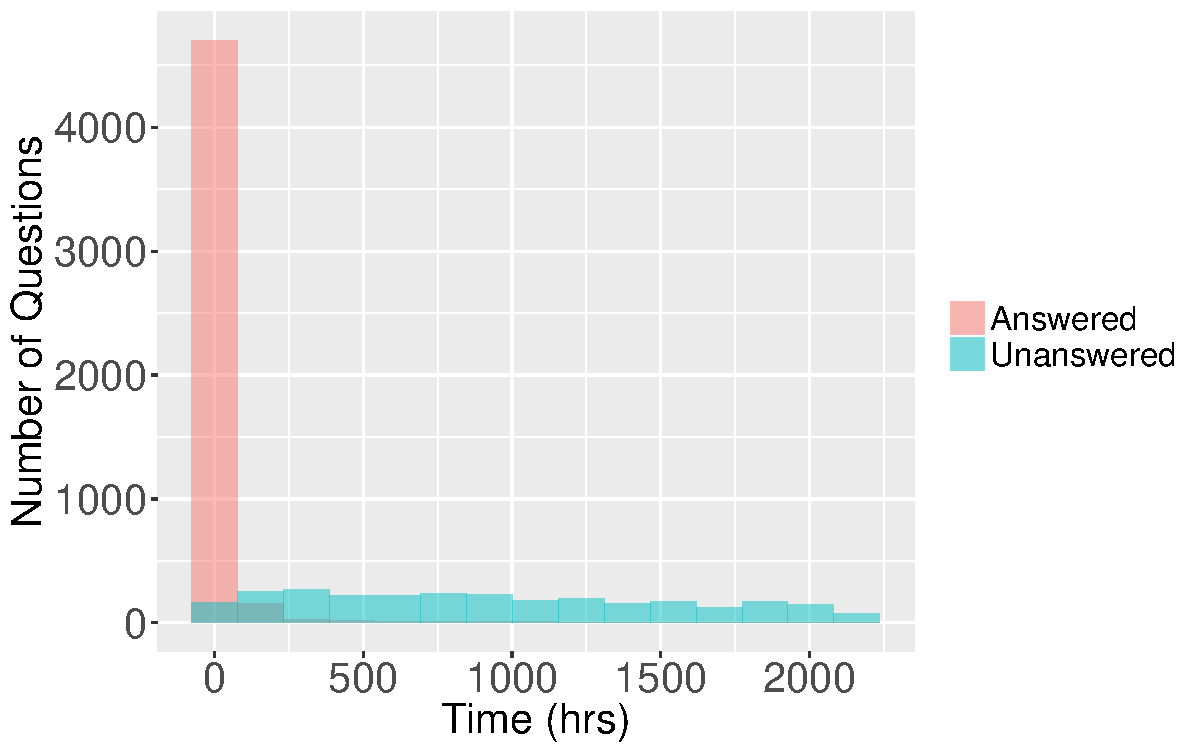
\includegraphics[width=1\linewidth]{FIG1.pdf}
\caption{Distribution of response times}
\label{fig1}
\end{figure}




%----------------------------------------------------------------------------------------

\end{column} % End of the first column

\begin{column}{\sepwid}\end{column} % Empty spacer column

\begin{column}{\onecolwid} % The first column

%----------------------------------------------------------------------------------------
%	METHODS
%----------------------------------------------------------------------------------------

\begin{figure}
\captionsetup{skip=25pt}
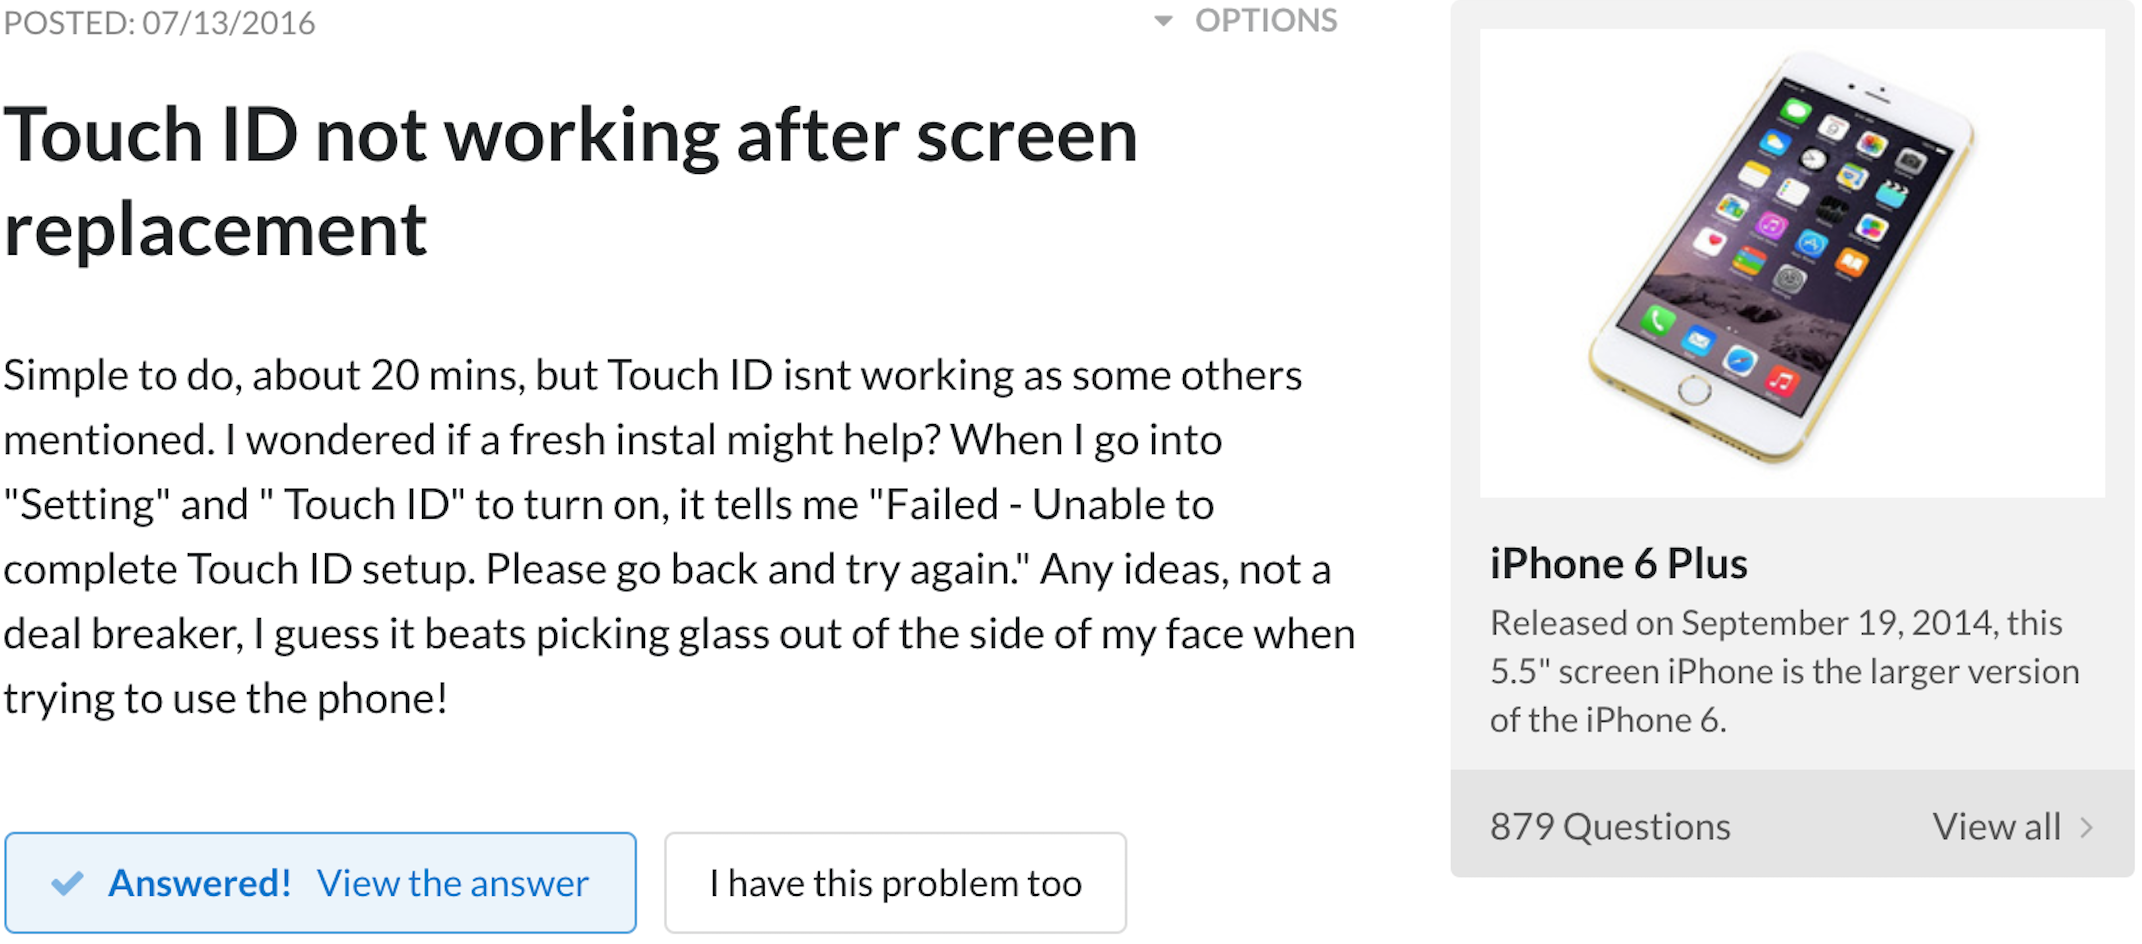
\includegraphics[width=1.08\linewidth]{question}
\caption{Example of a question posted on the forum}
\label{fig1}
\end{figure}

\vspace{2ex}

\begin{block}{Methods}

\textcolor{dblue!70}{\ding{228}} \textcolor{dblue!70}{\textbf{Univariate Analysis}} 

\vspace{0.25ex}

Used to identify which variables to include

\vspace{0.25ex}

\textcolor{dblue!70}{\ding{228}} \textcolor{dblue!70}{\textbf{Five Fold Cross-Validation}} 

\vspace{0.25ex}

Model was built on training sets and used to predict hazard ratios on test sets

\vspace{0.25ex}

Predicted hazard ratios were entered into separate Cox models; resulting metrics were averaged over each iteration and assessed

\vspace{0.25ex}

\textcolor{dblue!70}{\ding{228}} \textcolor{dblue!70}{\textbf{Final Model}} 

\vspace{0.25ex}

Model was fit to the full data and proportional hazards (PH) assumption was assessed

\vspace{2ex}

\end{block}

%----------------------------------------------------------------------------------------
%	RESULTS
%----------------------------------------------------------------------------------------

% \begin{block}{Cross-Validation Results}
% 
% \end{block}

\begin{table}[!htbp]
\captionsetup{skip=40pt}
\vspace{2.5ex}
\begin{tabular}{|r|r|r|r|r|r|r|r|}
  \hline
  & \textbf{HR} & \textbf{LR} & \textbf{p-value} & \textbf{$R^2$} & \textbf{\textit{Dxy}} & \textbf{C} \\
  \hline
  \textbf{Training} & 2.03 & 937.39  & \textless0.0001 & 0.14 & 0.27 & 0.63 \\
  \textbf{Test}     & 1.99 & 220.83  & \textless0.0001 & 0.14 & 0.26 & 0.63 \\
  \textbf{Full}     & 2.03 & 1165.03 & \textless0.0001 & 0.14 & 0.28 & 0.63 \\
  \hline
\end{tabular}
\caption{Performance metrics achieved in cross-validation and for the model fit to the full data (HR: Hazard Ratio, LR: Partial Likelihood Ratio, C: Concordance)}
\label{table:1}
\end{table}

\vspace{2.5ex}


\begin{block}{Final Model Statistics}

\textcolor{dblue!70}{\ding{228}} LR $=$ 1265.29 (p-value \textless0.0001)

\vspace{0.35ex}

\textcolor{dblue!70}{\ding{228}} $R^2 =$ 0.15

\vspace{0.35ex}

\textcolor{dblue!70}{\ding{228}} Somers' \textit{Dxy} $=$ 0.27

\vspace{0.35ex}

\textcolor{dblue!70}{\ding{228}} Device category violated the PH assumption

\end{block}

%----------------------------------------------------------------------------------------

\end{column} % End of the first column

\begin{column}{\sepwid}\end{column} % Empty spacer column

\begin{column}{\twocolwid} % Begin a column which is two columns wide (column 2)


%----------------------------------------------------------------------------------------

\begin{block}{Final Model Coefficients}
\end{block}

\begin{table}[!htbp]
\captionsetup{width=0.85\textwidth, skip=40pt}
\centering
\begin{tabular}{|L{10cm} L{17.5cm}|c|c|}
  \hline
 \textbf{Variable} & & \textbf{Coefficient (SE)} & \textbf{p-value} \\ \hline
  Device Category & Apple Product & 0.93 (0.048) & \textless0.0001 \\ 
                  & Camera & -0.32 (0.090) & \\ 
                  & Electronics & -0.01 (0.078)  & \\ 
                  & Game Console & 0.24 (0.083)  & \\ 
                  & Home & 0.34 (0.070) &  \\ 
                  & Other & -0.13 (0.056)  & \\ 
                  & PC & 0.28 (0.060) &  \\ 
                  & Tablet & -0.16 (0.081)  & \\ 
                  & Vehicle & 0.40 (0.069)  & \\
                  & Android/Other Phone (reference) & --- & \\ \hline
  \multicolumn{2}{|l|}{Weekend} & -0.13 (0.033)  & \textless0.0001 \\ \hline
  \multicolumn{2}{|l|}{Text contains end punctuation} & 0.03 (0.050) & 0.613 \\ \hline
  \multicolumn{2}{|l|}{Text is in all lower case} & -0.18 (0.064) &  0.006 \\ \hline
  \multicolumn{2}{|L{30cm}|}{Title contains terms considered frequently-used among answered questions} & 0.05 (0.042) &  0.260 \\ \hline
  \multicolumn{2}{|L{30cm}|}{Title contains terms considered frequently-used among unanswered questions} & -0.28 (0.034)  & \textless0.0001 \\ \hline
  \multicolumn{2}{|L{30cm}|}{Title ends in a question mark} & 0.26 (0.033) &  \textless0.0001 \\ \hline
  \multicolumn{2}{|L{30cm}|}{User edited or added to the question's text after posting it} & 0.30 (0.086)  & 0.001 \\ \hline
  \multicolumn{2}{|L{30cm}|}{User was a member for less than one day before posting} & -0.11 (0.036)  & 0.003 \\ \hline
  \multicolumn{2}{|L{30cm}|}{User made an effort to solve the problem prior to asking the question} & -0.07 (0.036)  & 0.045 \\ \hline
  \multicolumn{2}{|L{30cm}|}{Square root of the average tag frequency} & 2.23 (0.720)  & 0.002 \\ \hline
\end{tabular} 
\caption{Not shown: continuous predictors fit with restricted cubic splines (text length, average tag length, device name length, ratio of number of newlines to text length)} 
\end{table}


%----------------------------------------------------------------------------------------


\begin{columns}[t,totalwidth=\twocolwid] % Split up the two columns wide column again

\begin{column}{\onecolwid} % The first column within column 2 (column 2.1)


\begin{block}{Select Interpretations}

Controlling for all other predictors, the estimated hazard of receiving an answer is:

\vspace{1ex}

\textcolor{dblue!70}{\ding{228}} 154\% higher (95\% CI (132\%, 179\%)) for Apple products vs. Android/other phones

\vspace{1ex}

\textcolor{dblue!70}{\ding{228}} 13\% lower (95\% CI (7\%, 18\%)) for questions posted on the weekend vs. weekday

\vspace{1ex}

\textcolor{dblue!70}{\ding{228}} 25\% lower (95\% CI (19\%, 29\%)) for questions with titles containing at least one frequently-used word among unanswered question titles vs otherwise

\end{block}

%----------------------------------------------------------------------------------------

\end{column} % End of column 2.1

\begin{column}{\onecolwid} % The second column within column 2 (column 2.2)

\begin{block}{Forum Design Suggestions}

\textcolor{dblue!70}{\ding{228}} Rather than allowing users to enter any tag or device name, restrict options to a drop-down list

\vspace{0.75ex}

\textcolor{dblue!70}{\ding{228}} Include tips to guide users asking questions 

\end{block}

\vspace{1ex}

\begin{block}{Acknowledgements}

\textcolor{dblue!70}{\ding{228}} Research was supported by the Bill and Linda Frost fund of California Polytechnic State University, San Luis Obispo. We also thank iFixit for providing access to the \textit{Answers} data.

\end{block}

%----------------------------------------------------------------------------------------

\end{column} % End of column 2.2

\end{columns} % End of the split of column 2

\end{column} % End of the second column

% \begin{column}{\sepwid}\end{column} % Empty spacer column



%----------------------------------------------------------------------------------------

%----------------------------------------------------------------------------------------
%	ACKNOWLEDGEMENTS
%----------------------------------------------------------------------------------------

% \setbeamercolor{block title}{fg=red,bg=white} % Change the block title color

% \begin{block}{Acknowledgements}
% 
% \small{\rmfamily{This research was supported by the Bill and Linda Frost fund of the California Polytechnic State University of San Luis Obispo. We also thank iFixit for providing access to the CQA data.}} \\
% 
% \end{block}
% 
% \end{column} % End of the third column
% 
\end{columns} % End of all the columns in the poster

\end{frame} % End of the enclosing frame

\end{document}
